\subsection{Forecast residuals and control performance}


\begin{figure}[!ht]
\centering
  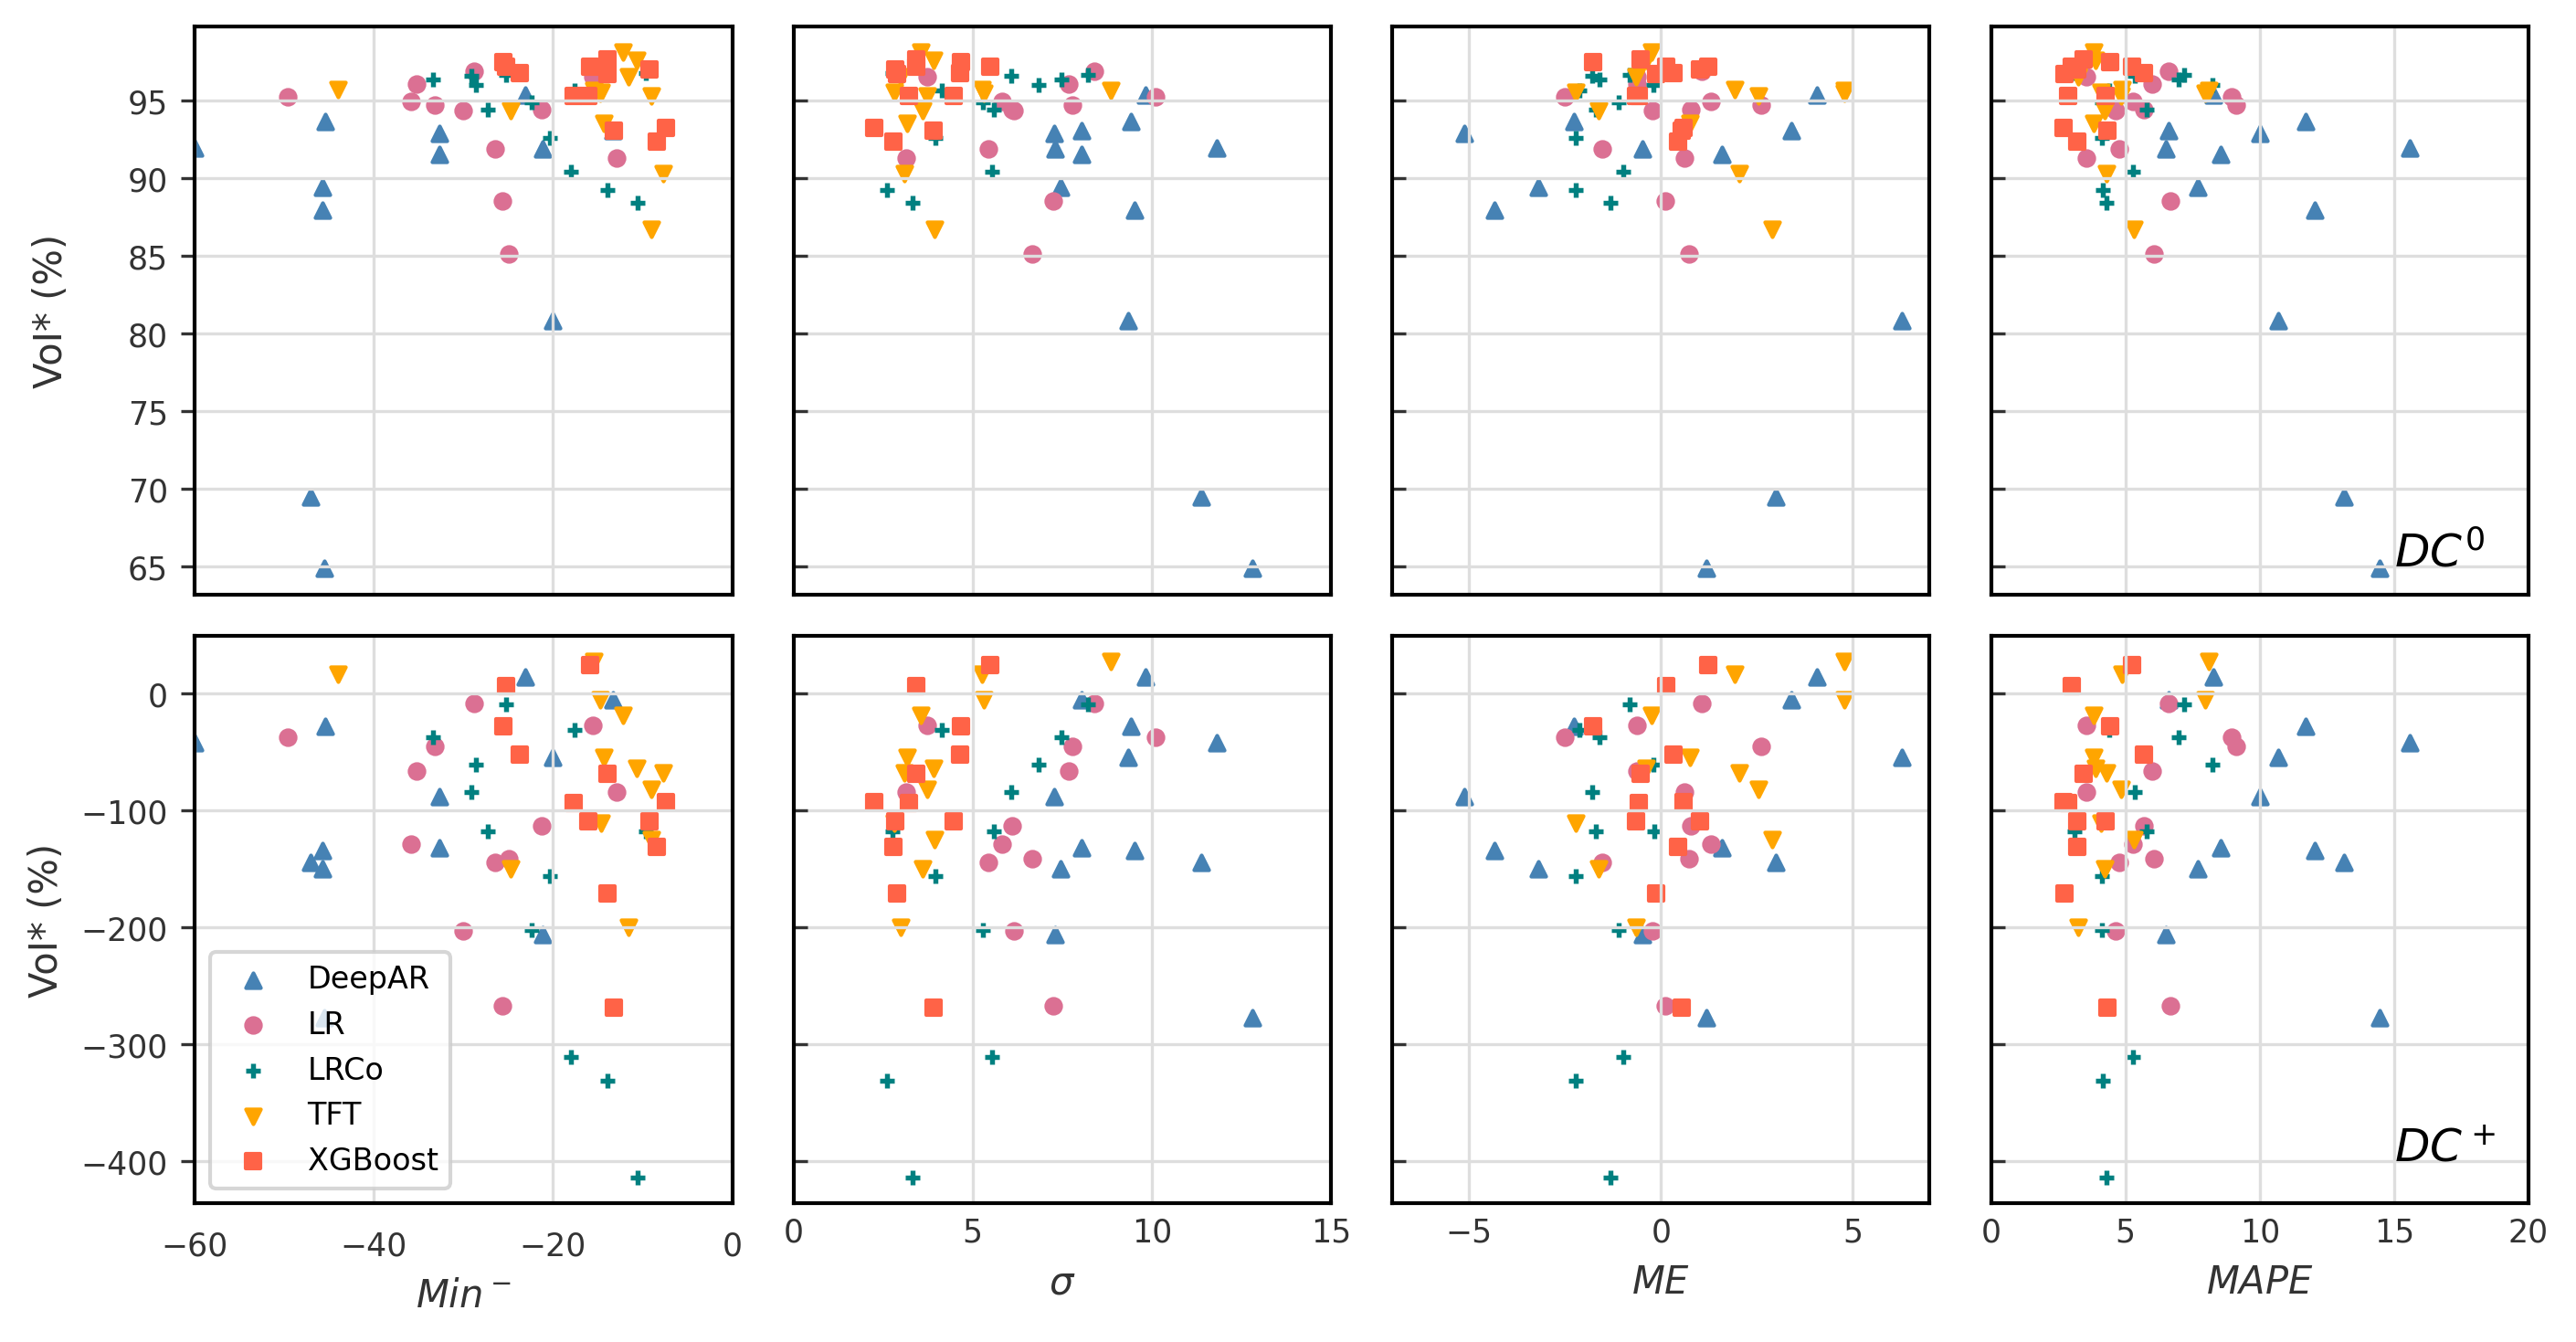
\includegraphics[width=1\textwidth]{figures/fig-10-VoI-metrics-pair-plot-2.png}
  \caption{\textit{} $x$-axis is values of metrics differed in each column. $y$-axis is the corresponding normalized value of information (VoI*). Each marker represents one monthly trial. Different forecast models are marked by varied markers. }
  \label{fig:VoI-metrics}
\end{figure}


\begin{figure}[!ht]
\centering
  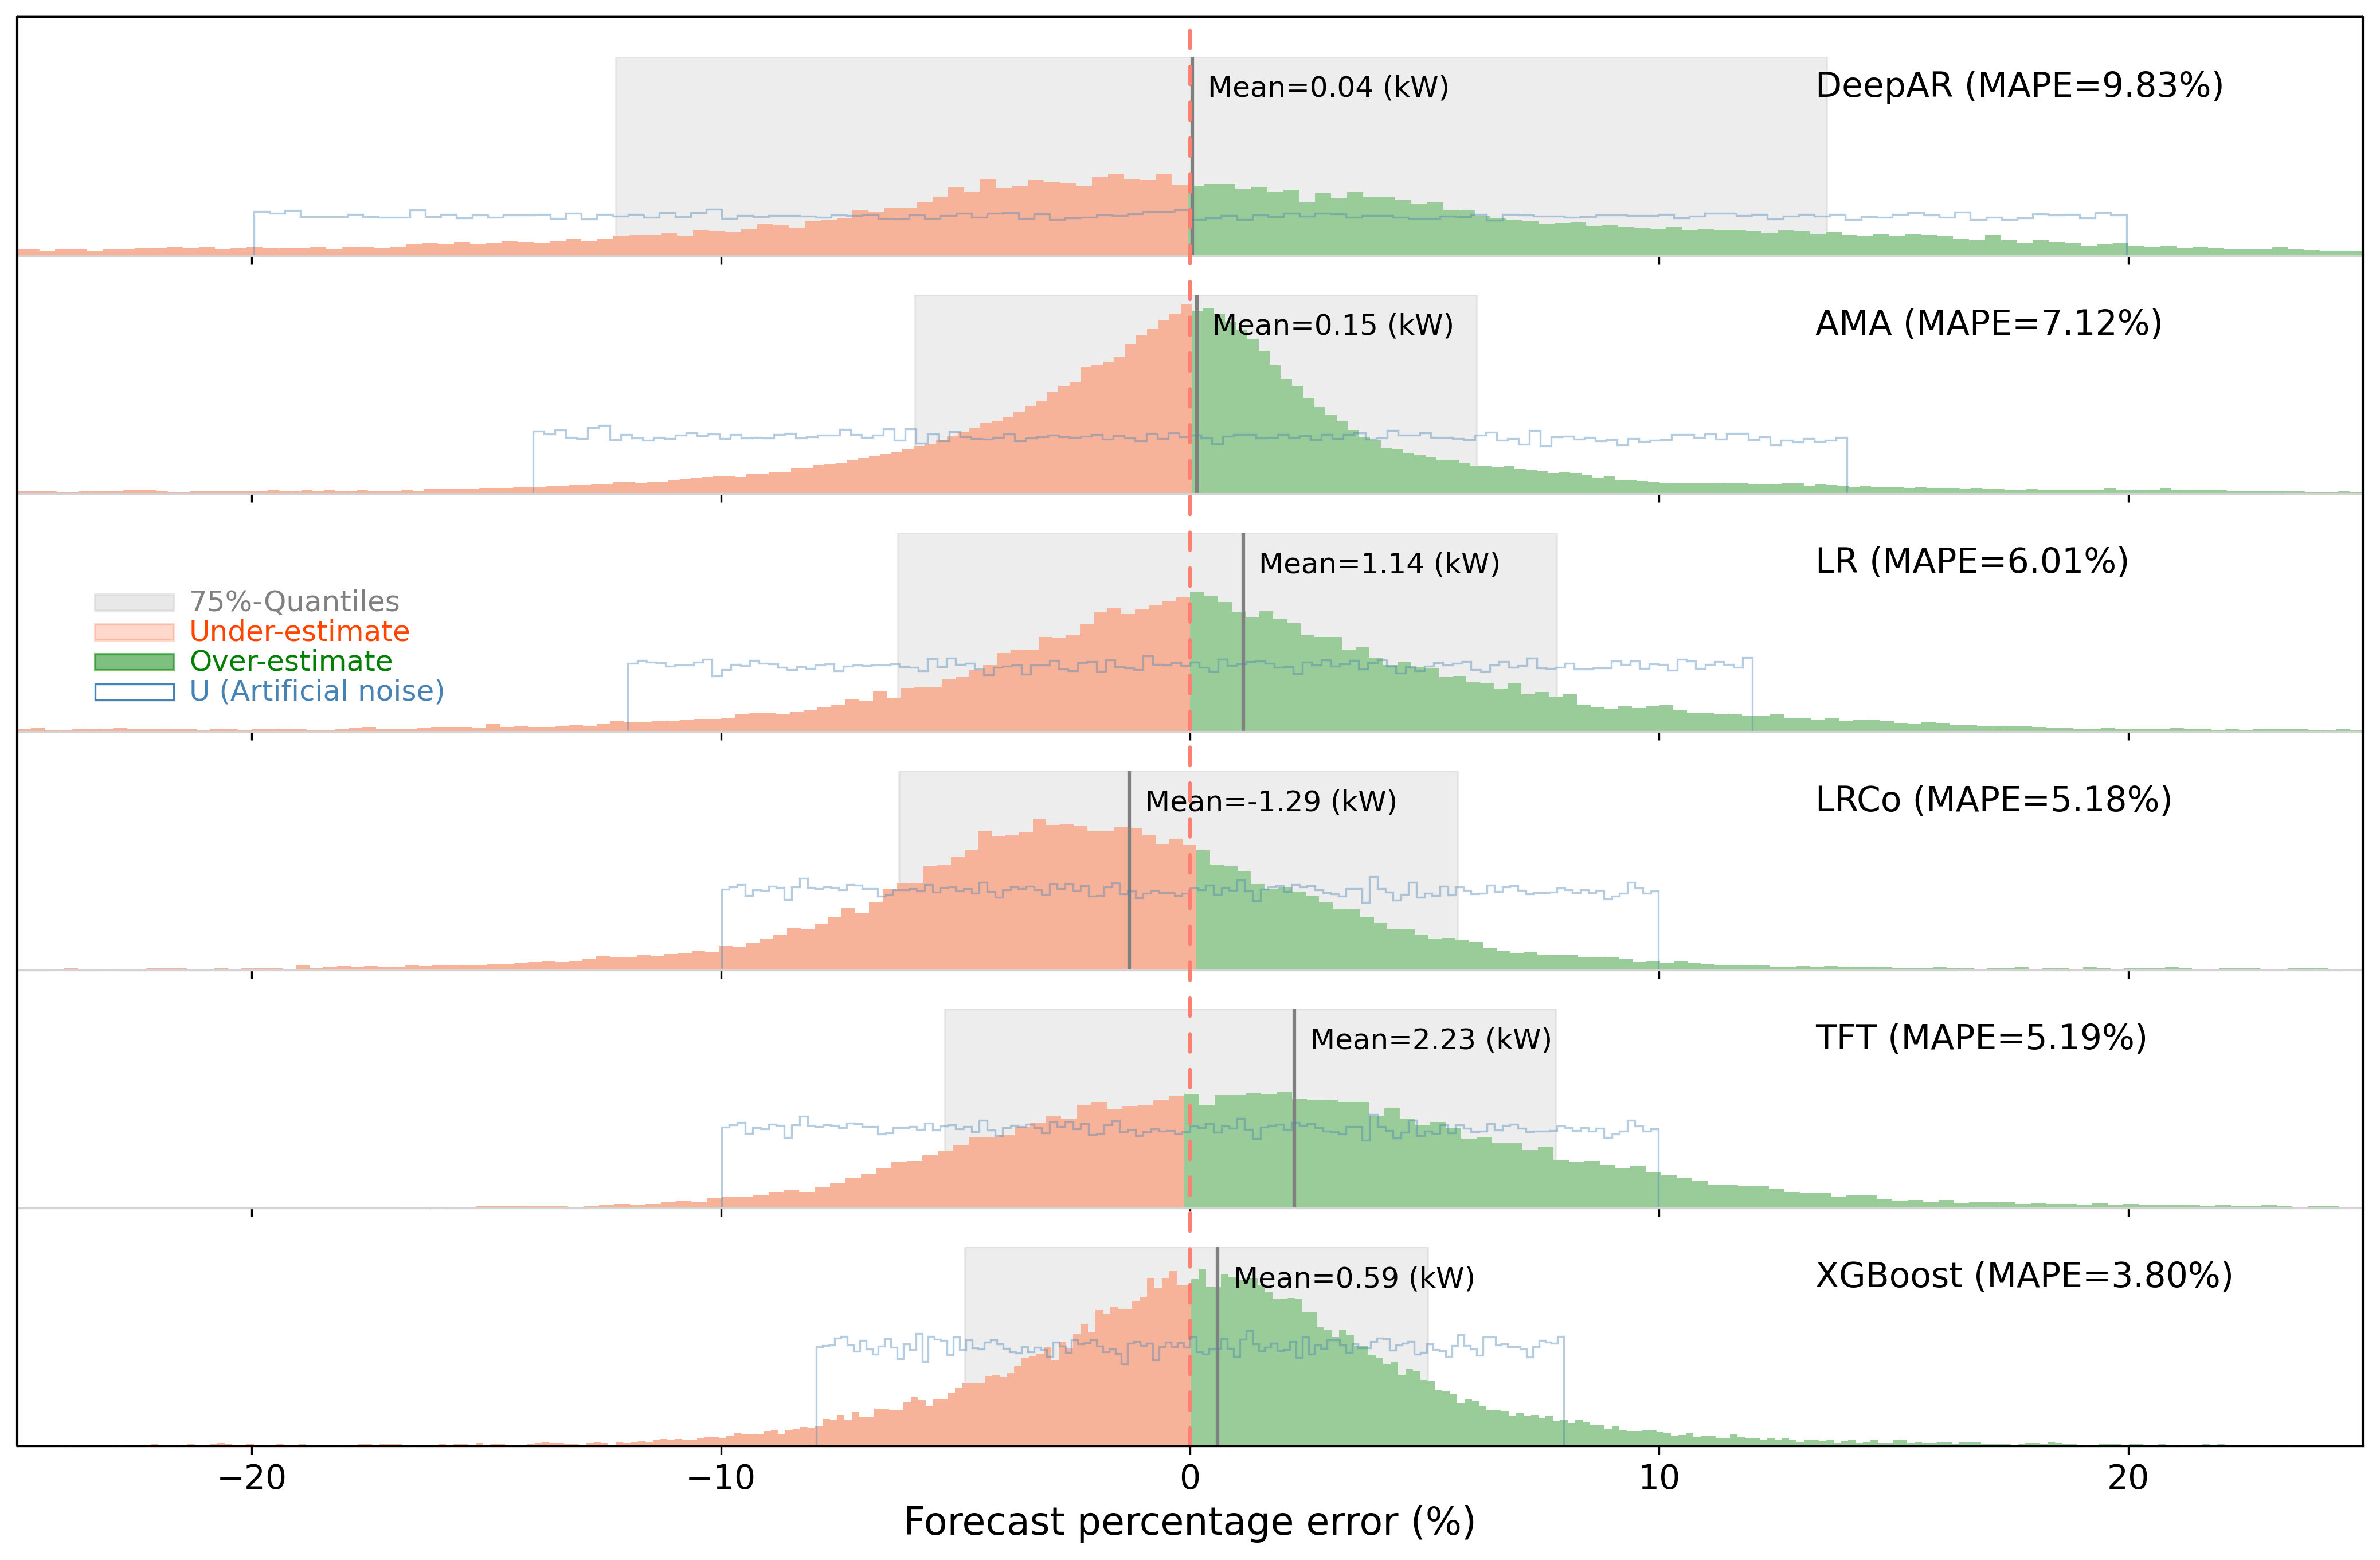
\includegraphics[width=0.85\textwidth]{figures/fig-7-residual-all.png}
  \caption{\textit{Forecast error distribution compared with artificial noise ($\textbf{U}$).} $x$-axis shows the value of forecast percentage error. Histogram in each subplot shows the error distribution of one specific prediction model tagged in the upper right. Orange bars are underestimated part, and green ones are overestimated part. Gray shading area marks the 75\% percentiles of the distribution. Mean value of forecasting errors is tagged. For comparison, the error distribution of unbiased artificial noise ($\textbf{U}$) is plot with blue lines, and corresponding magnitude, namely MAPE, is close to that of the model in the same subplot.}
  \label{fig:Error-distb-SOTA}
\end{figure}

The preceding observations suggest that the MAPE may not effectively serve as an adequate indicator of MPC's performance, especially when considering demand charges. Therefore, we incorporated three additional metrics that encapsulate aspects of the \emph{worst-case} scenario, \emph{variance}, and \emph{magnitude of mean values} for forecast residuals, as outlined in Eqs. (\ref{eq:Min-}) to (\ref{eq:ME}), where $\widehat{y_t}$ and $y_t$ represent the forecasted and actual values, respectively. The minimum value of underestimation:

\begin{equation} \label{eq:Min-}
    Min^- = min \{\widehat{y_{t}}-y_{t}|0<t<n \}
\end{equation}
The standard deviation $\sigma$ indicating the fluctuation of residuals:
\begin{equation} \label{eq:Std}
    \sigma=\sqrt{\frac{1}{n}{\sum_{k=1}^n (\widehat{y_t}-\bar{y})^2}}
\end{equation}
The average value of forecasting errors:
\begin{equation} \label{eq:ME}
    ME = \frac{1}{n} \sum_{t=1}^{n} (\widehat{y_{t}}-{y_{t})}
\end{equation}
%\begin{equation} \label{eq:MAE-}
%    ME^- = \frac{1}{n} \sum_{t=1}^{n} min\{0,{y_{t}-\widehat{y_{t}}}\}
%\end{equation}

In order to observe more samples, we present the monthly values individually, as depicted in Figure \ref{fig:VoI-metrics}. Notably, our chosen metrics exhibit a rather significant correlation with the VoI* metric under $\wodc$, with $\sigma$ and MAPE revealing a discernible relationship. However, under $\wdc$, increased uncertainties obscure such correlations, with only the ME metric indicating that higher ME values tend to correspond to higher VoI* outcomes.

Moreover, analyzing the distribution of forecast residuals may provide more insightful information for interpreting the influence of forecast errors, as shown in Fig. \ref{fig:Error-distb-SOTA}. It is evident that the forecast residuals distribute normally and have a more centralized distribution compared to artificial noise. 
%The superior control performance of MPC-ML over \MPCe may be attributed to such differences.
Additionally, there are variations in the distribution pattern among different forecasts. DeepAR , AMA and XGBoost exhibit relatively symmetrical distribution.
%though XGBoost indicates a more centralized distribution that corresponds with the MAPE.  
TFT and LR demonstrate a greater amount of residuals in the overestimated section, clarifying why \textbf{MPC-TFT} and \textbf{MPC-LR} exceed performance expectations. This is attributed to overestimated forecasts shown to perform better under $\wdc$, as analysed in Sec. \ref{sec:Asymmetric impact}. LRCo, in contrast, have more underestimated residuals, thus \textbf{MPC-LRCo} exhibits performance inferior to TFT which has similar MAPE. 


These observations highlight the need for the development of synthesized error metrics to more comprehensively uncover the intricate relationship between forecast residuals and MPC control performance within the domain of microgrid management. Singular and lump metrics, while informative, can capture only a single dimension of the residual characteristics. Other factors tied to time series patterns hold greater significance for MPC control challenges, as they exert a direct influence on the execution stage of MPC strategies. Our future research endeavors will be dedicated to further exploring and elucidating these relationships.

%In this section, it is concluded that both centralizing forecast residuals and overestimation are beneficial for MPC in terms of control performance. Centralizing the residuals takes the leading role under $\wodc$, whereas under $\wdc$, overestimation significantly improves control performance due to the biased impact of forecast error.

\subsection{Value of forecasts in the scope of time}

\begin{figure}[!ht]
\centering
  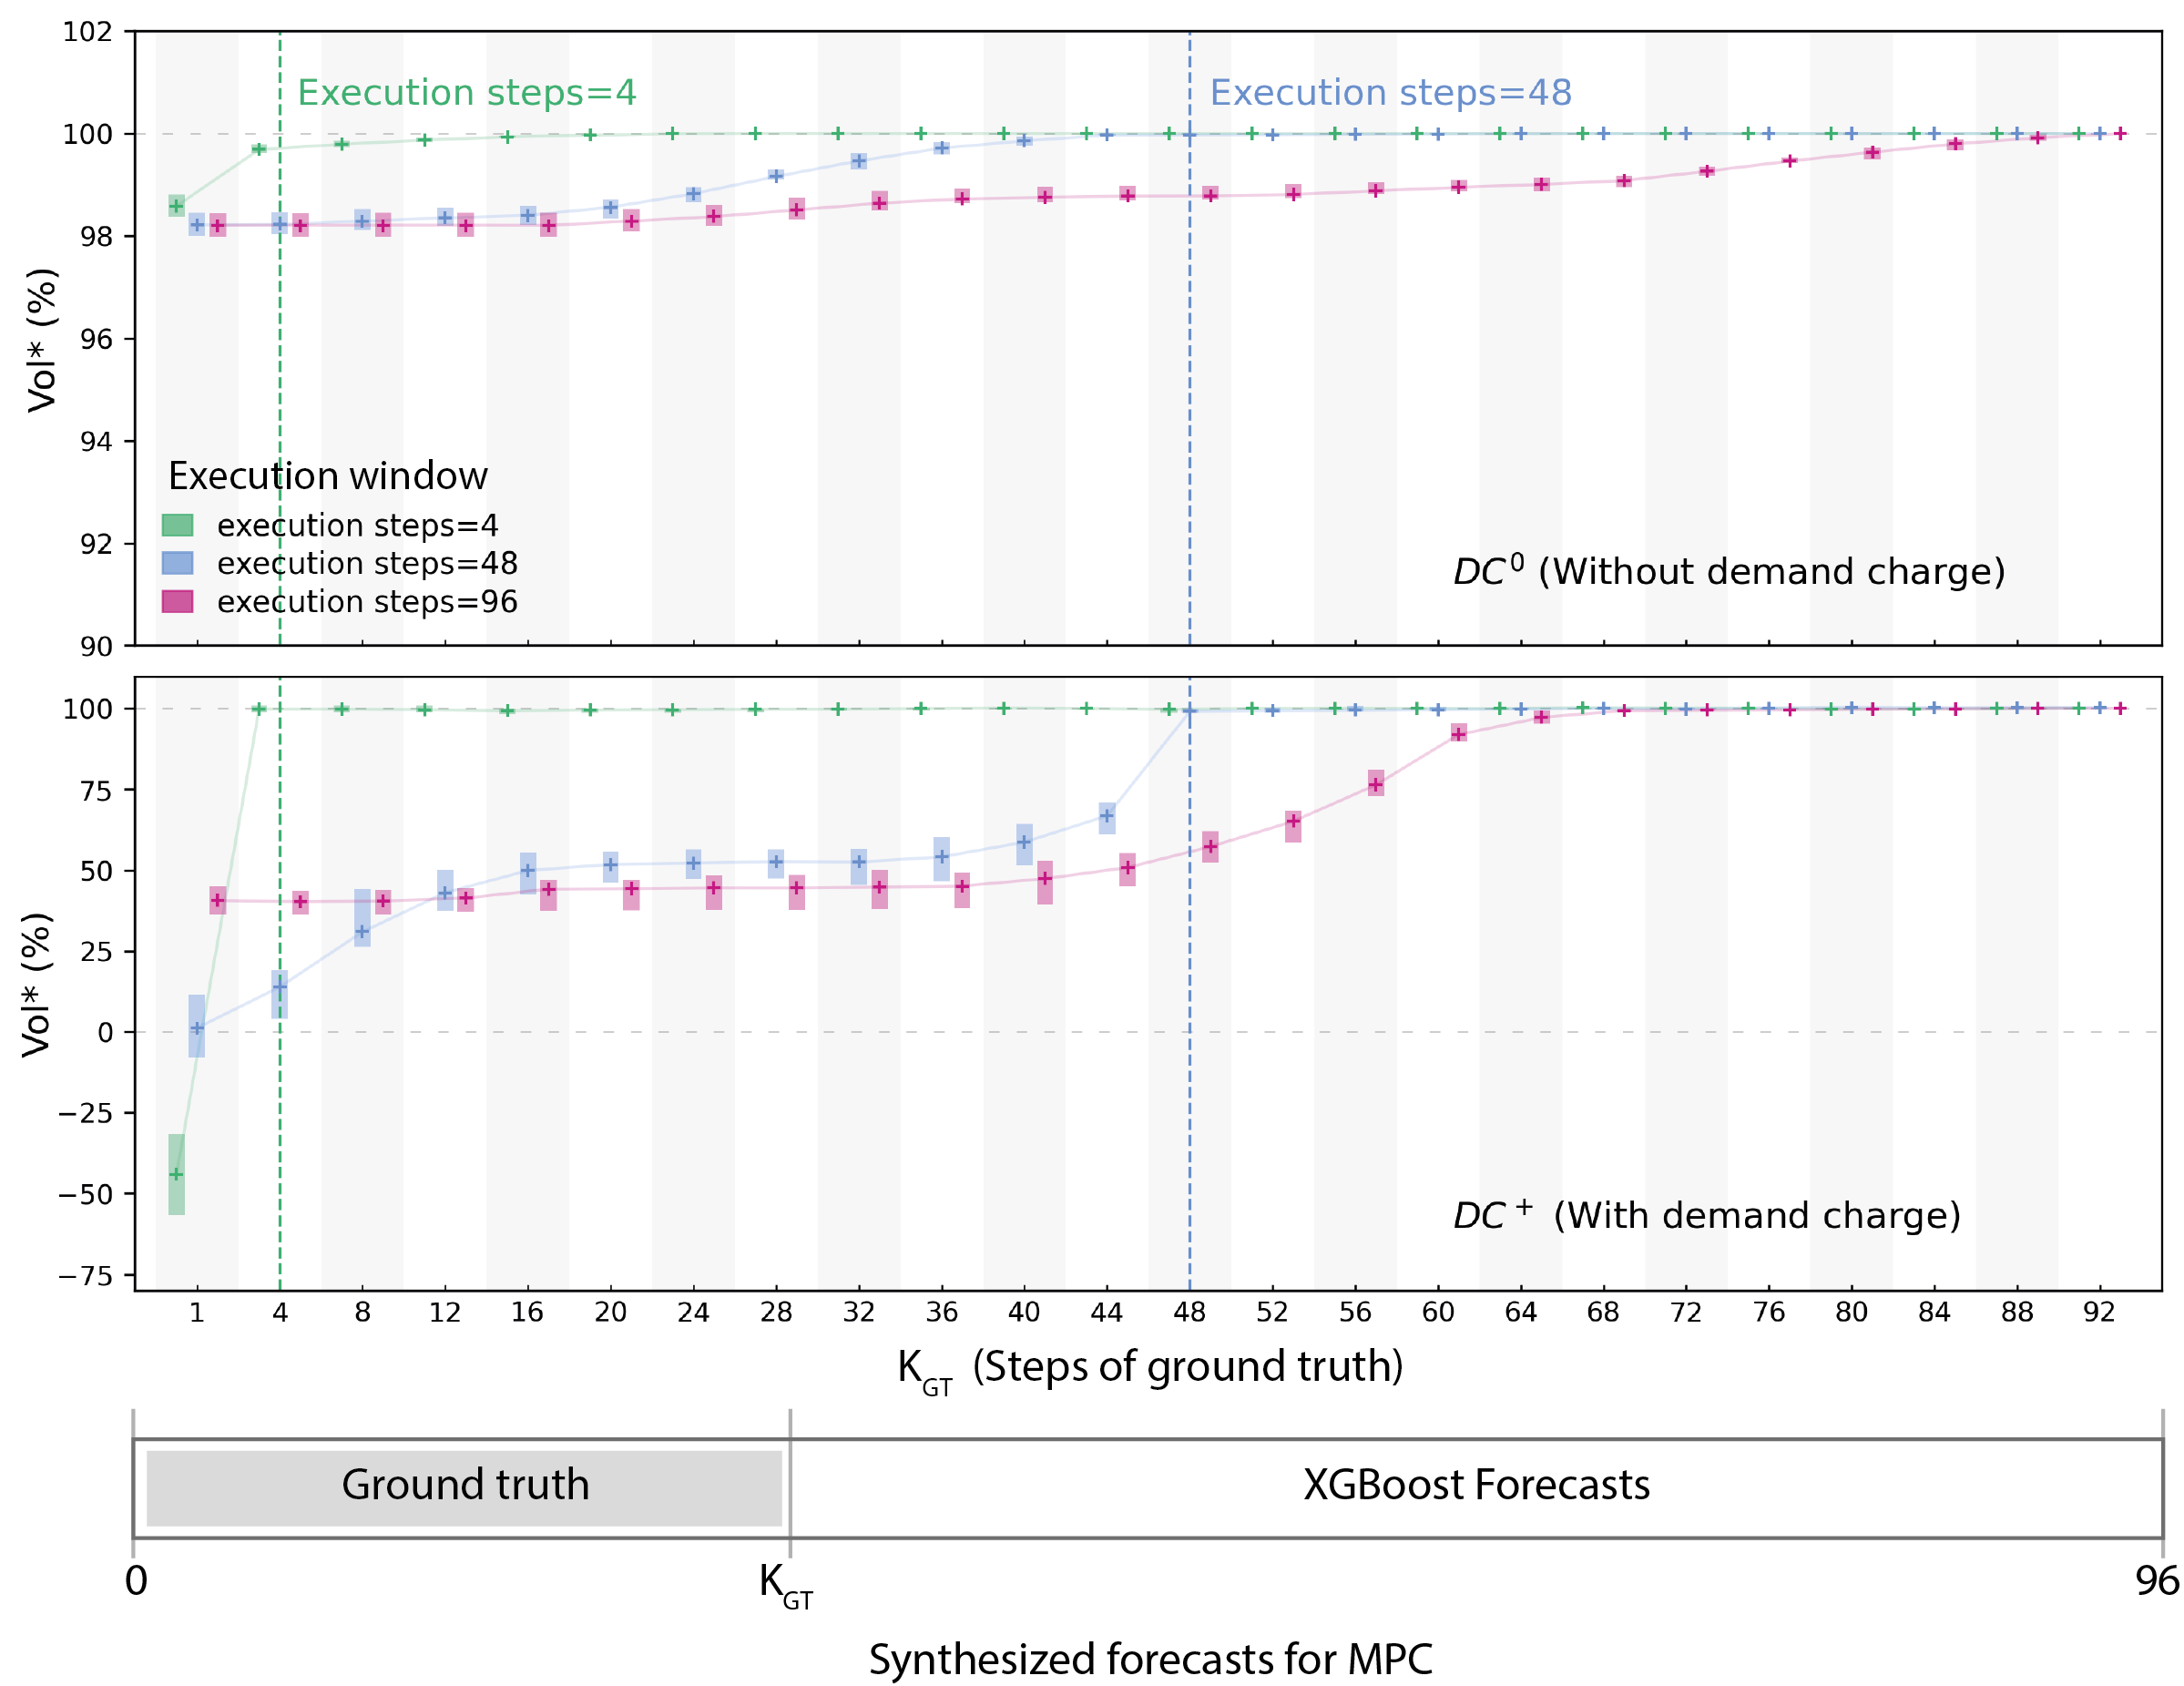
\includegraphics[width=0.85\textwidth]{figures/VoI_timescope.png}
  \caption{\textit{VoI* with varied forecast in time-scope.} $x$-axis is the steps of ground truth given to each CFTOC problem. How the forecasts are concatenated is shown in the diagram at the bottom. $y$-axis is the corresponding normalized value of information (VoI*). Each bar marks the 25\% and 75\% percentiles of trials for 12 months in 2019, and "+" marks their mean values. }
  \label{fig:VoI-timescale}
\end{figure}

In this study, the MPC optimization is a dynamic process. Within a single control window, K steps of forecasts are considered in the linear programming (LP), and only $\kexe$ steps of solutions are executed\footnote{In this study, K is set as 96 and $\kexe$ is 4, which correspond to 24h and 1h.}. Consequently, it is pertinent to examine the value of the prediction over time. A straightforward approach would be to create a combined prediction by merging accurate data with forecasts. As shown in Fig. \ref{fig:VoI-timescale}, we concatenate ground truth $\{\pbld_{t} \mid 0\leq t \leq \kgt\}$ and forecasts $\{\bldest_{t} \mid \kgt< t < K\}$ as synthesized forecasts for each step, and then conduct monthly simulations in 2019 while varying $\kgt$ between 0 and 96. The simulations were conducted in three groups for $\kexe$ values of 4, 48, and 96, as depicted by three colors.

The key observation is that the forecast error taking place within the execution window exerts a significant impact on control performance, compared to the negligible influence of errors occurring outside this window. This is because forecasts beyond the execution window help the LP detect and adapt to future trends, and associated errors do not have a direct effect on control performance. In contrast, forecast errors occurring within the execution window cause a direct mismatch between the solutions and executions, resulting in sub-optimality. 

Furthermore, there is another phenomenon that is somewhat counter-intuitive. In the case of $\wodc$, frequent re-optimization yields better performance as expected albeit with limited improvement. However, under $\wdc$, frequent re-optimization leads to deteriorating control performance. As depicted in Fig. \ref{fig:VoI-timescale}, when $\kgt$ is 1 and under $\wdc$, MPC with execution window of 96 steps (purple bars) outperform that with 4 steps (green bars). As examined in Sec. \ref{sec:Asymmetric impact}, frequent re-optimisation leads to offering inaccurate information more frequently. Therefore, decreasing the frequency of optimization when highly-accurate forecasts are unavailable under $\wdc$ refines performance control and diminishes the computational load.



